\section{Analysis}
\label{sec:analysis}

The two fixes from Section~\ref{sec:v2} are independently small but jointly load-bearing. This section explains why each one matters and what the gate ends up doing during training.

\subsection{The gate stays alive in v2}

\begin{figure}[H]
    \centering
    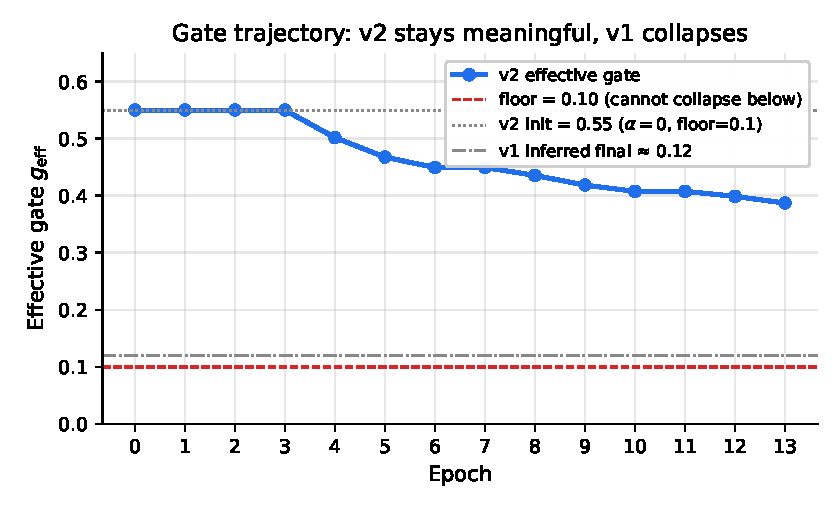
\includegraphics[width=0.78\textwidth]{figures/gate_evolution.pdf}
    \caption{Effective gate $g_{\mathrm{eff}}$ across training. v2 drifts gradually downward from $0.55$ to ${\approx}0.39$ over $13$ epochs, settling well above the $0.10$ floor. v1's gate, estimated from a checkpoint, sat at ${\approx}0.12$ for most of training.}
    \label{fig:gate-evolution}
\end{figure}

Figure~\ref{fig:gate-evolution} shows the effective gate over time. With the floor in place, the optimizer is free to attenuate the feedback signal and does so partially (the gate does not stay at $0.55$), but it cannot drive the gate to zero. By epoch~$12$, the gate sits at $0.39$ --- meaning roughly $39\%$ of the cross-attention output flows back into memory at every forward pass. v1's gate by the same point of training was ${\approx}0.12$, below what we set as v2's floor; the v1 ablation showed exactly this silence.

\subsection{Role of the floor}

Without a floor, the optimizer has a costless escape: pushing $\alpha$ further negative reduces a noisy signal during training, and the rest of the network adapts around the resulting zero feedback. The floor reparameterization removes this escape route. Crucially, it does not force the gate to be high --- the optimizer can still learn an attenuation pattern --- it only prevents the contribution from being driven to zero. That is enough to keep the cross-attention causally relevant at inference.

\subsection{Role of the level mask}

A single set of cross-attention weights cannot simultaneously be optimal for stride-4 tokens (where small objects are sub-pixel-precise) and for stride-32 tokens (where each token covers a $32{\times}32$ neighborhood). v1 forced the same mechanism to do both. v2 specializes: it only refines P2 and P3, where small-object information lives. This is the same locality-prior that motivates feature pyramids in the first place~\cite{lin2017fpn}; we extend it to the feedback path.

\subsection{The two fixes are complementary}

The floor keeps the gate alive. The mask makes the alive-gate's signal targeted. Stripping either change should revert the mechanism toward silence: without the floor, the gate decays; without the mask, the attention pattern is split across irrelevant token regimes. We did not run the targeted $2{\times}2$ ablation that would isolate floor-only and mask-only effects (Section~\ref{sec:limitations}); that is the natural next experiment.
